\documentclass{beamer-control}
\usepackage{beamer-control-singlefile}
\INCLUDEONLY{Modeling Uncertainty}
\begin{document}
\CONCEPT{Modeling Uncertainty}

\begin{SUMMARY}
\begin{itemize}
\item Types of uncertainty
\item Similarity
\end{itemize}
\vfill References:
\begin{itemize}
\item \astrom{§13.1}
\end{itemize}
\end{SUMMARY}



\SUBCONCEPT{Types of uncertainty}

\begin{frame}{Parametric uncertainty}
\begin{itemize}
\item We would like our control systems to be robust to uncertainty 
\item One form of model uncertainty is \textit{parametric uncertainty}, when we do not have precise knowledge of the parameters describing a system
\item The parameters that describe the linearisation of nonlinear systems depends on the operating point, and hence may also be subject to uncertainty
\item A simple example of parametric uncertainty is when we do not know the mass of a car (which may vary due to number of passengers and weight of baggage) for cruise control
\end{itemize}
\end{frame}

\begin{frame}{Cruise control example}
\begin{itemize}
	\item Consider a PI controller designed for a nominal operating condition of mass $m=1600$kg for the cruise control system
	\item The figure below shows the results of encountering a slope of $4^\circ$ with masses in the range $1600<m<2000$ 
\end{itemize}
\begin{figure}
	\centering
	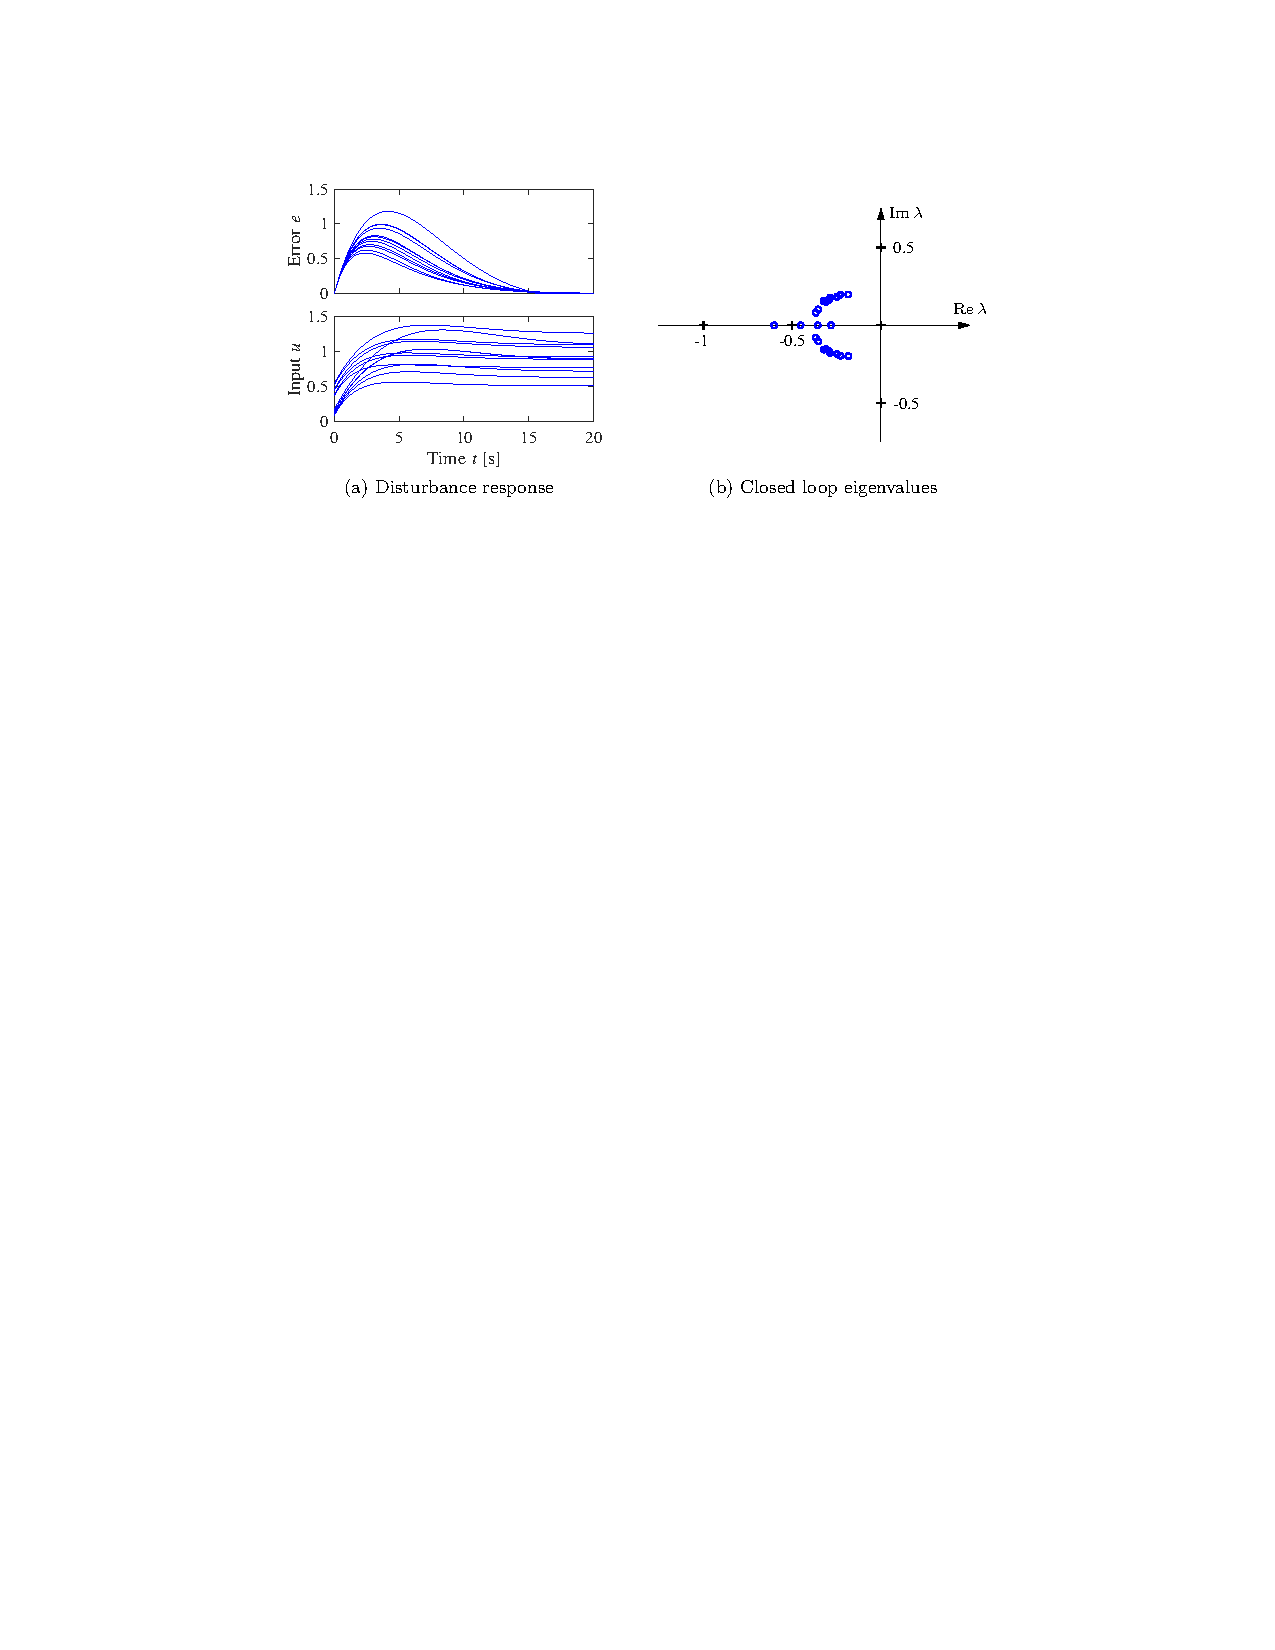
\includegraphics[width=9cm]{figure13.1}\\
	\vspace{-0.2cm}
	\textbf{Figure 13.1:} Responses of the cruise control system.
\end{figure}
\end{frame}


\begin{frame}{Unmodeled dynamics}
\begin{itemize}
\item We may easily investigate the effects of variations in parameters but other uncertainties must also be considered
\item For example, the cruise control system fails to account for the dynamics of the engine combustion processes, nonlinear air resistance, or delays between applying the throttle and the force at the wheels
\item These negelected mechanisms are known as \textit{unmodeled dynamics}
\item One approach is to make our model more complex but this can be challenging and often introduces more parameter uncertainty
\item We may instead probe our system to see if it is sensitive to generic forms of unmodeled dynamics
\end{itemize}
\end{frame}


\begin{frame}{Describing unmodeled dynamics}
	\begin{itemize}
		\item The nominal model may be augmented by a bounded input/output transfer function that captures the generic features of the unmodeled dynamics (additive $\Delta$, multiplicative $\delta$, or feedback uncertainty $Delta_{fb}$)
		\item These types of  are related by
		\[\delta=\frac{\Delta}{P}, \quad \Delta_{fb} = \frac{\Delta}{P(P+\Delta)}=\frac{\delta}{P(1+\delta)}\]
		\item If the closed loop system is stable for \textit{all}  bounded input/output transfer functions, the system is said to be robustly stable
		
	\end{itemize}
\begin{figure}
	\centering
	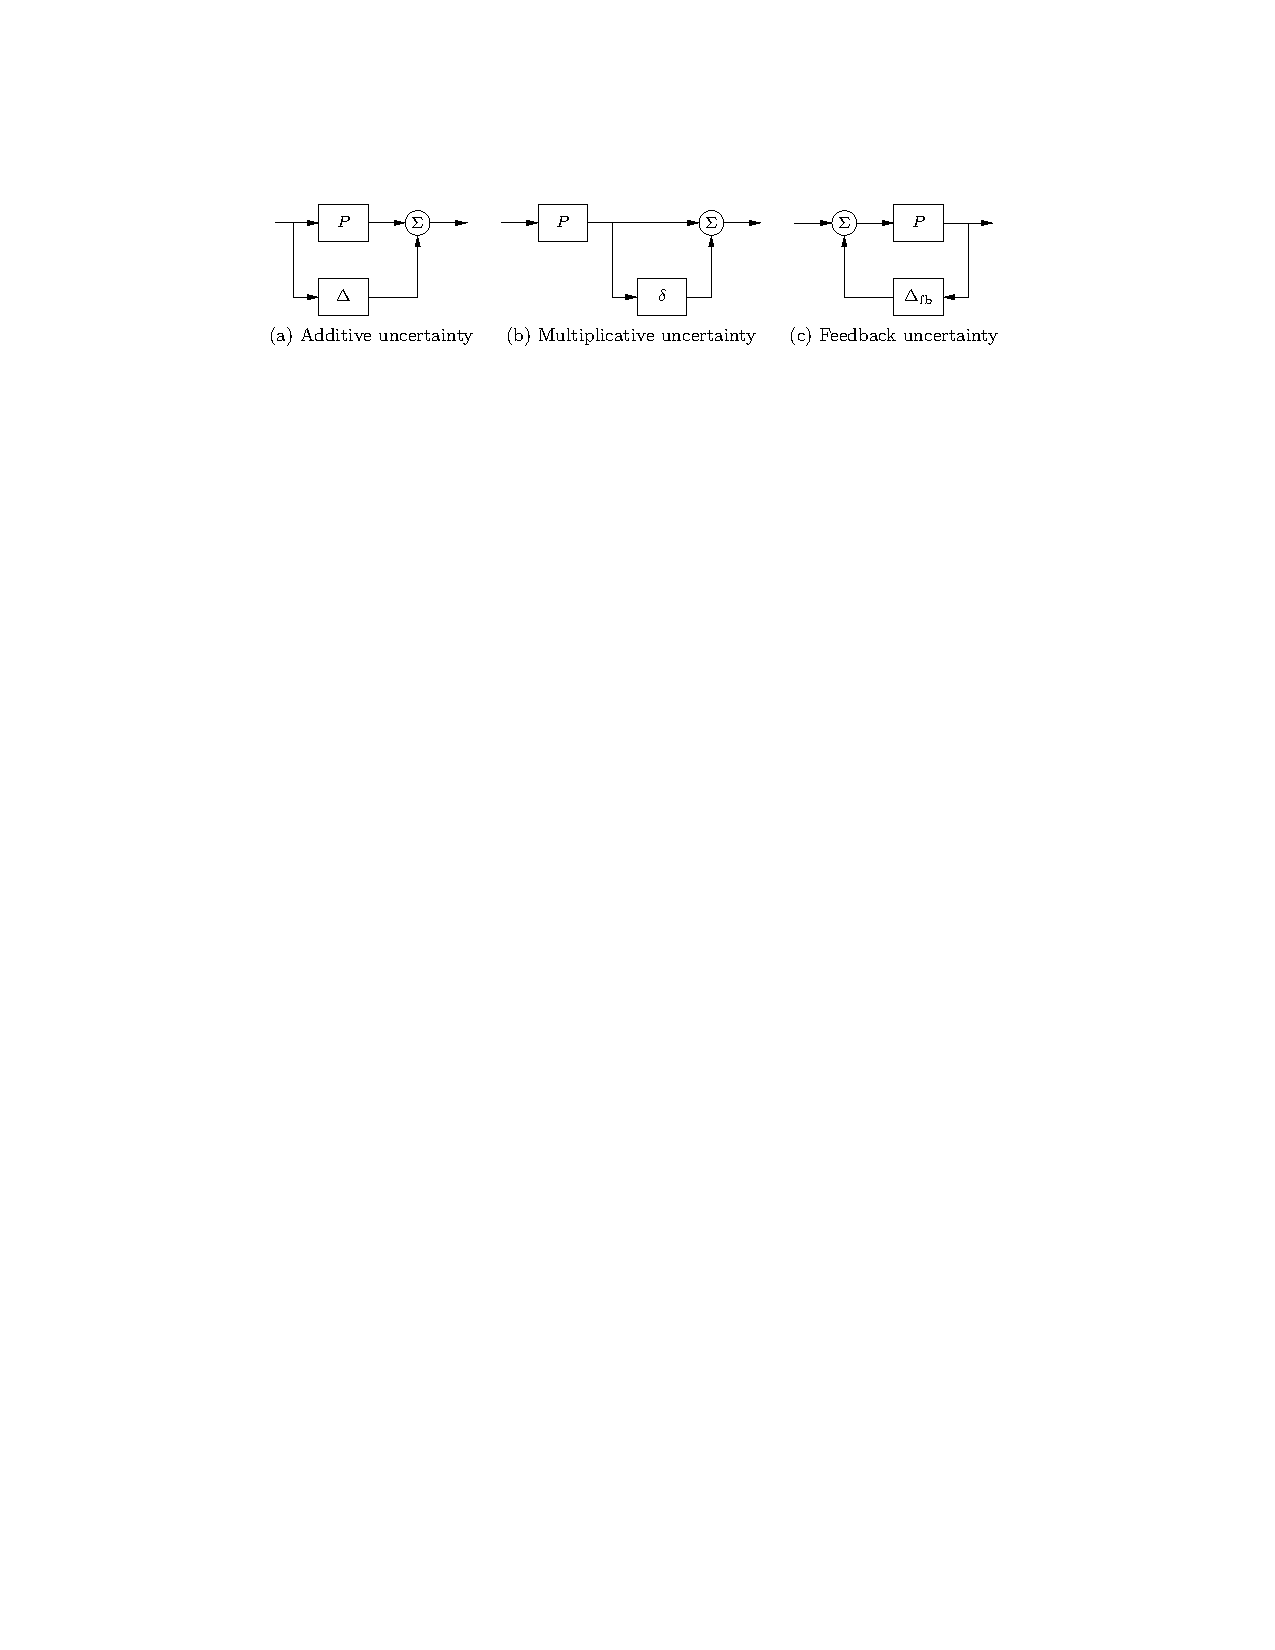
\includegraphics[width=10cm]{figure13.2}\\
	\vspace{-0.2cm}
	\textbf{Figure 13.2:} Unmodeled dynamics in linear systems.
\end{figure}
\end{frame}


\SUBCONCEPT{Similarity}

\begin{frame}{When are two systems similar?}
	\begin{itemize}
		\item It would be very useful to have a method to determine when two systems are close
		\item We need to be careful, as only comparing systems by their open loop behaviour (step responses and frequency responses) gives misleading results
		\item Let us look at two such examples
		\item The Vinnicombe metric is the proper way to compare open loop systems in a way that reflects closed loop behaviour, but we will not cover it here 
	\end{itemize}
\end{frame}


\begin{frame}{Examples}
\begin{itemize}
	\item Consider the transfer functions 
	\[P_1(s)=\frac{k}{s+1},\quad P_2(s)=\frac{k}{(s+1)(sT+1)^2} \] 
	\item These give seemingly identical open loop step responses for very small values of $T$
	\item Closing the loop with unit gain and plotting the closed loop step response shows that the first system is stable in closed loop and the second is unstable
	
\end{itemize}
\begin{figure}
	\centering
	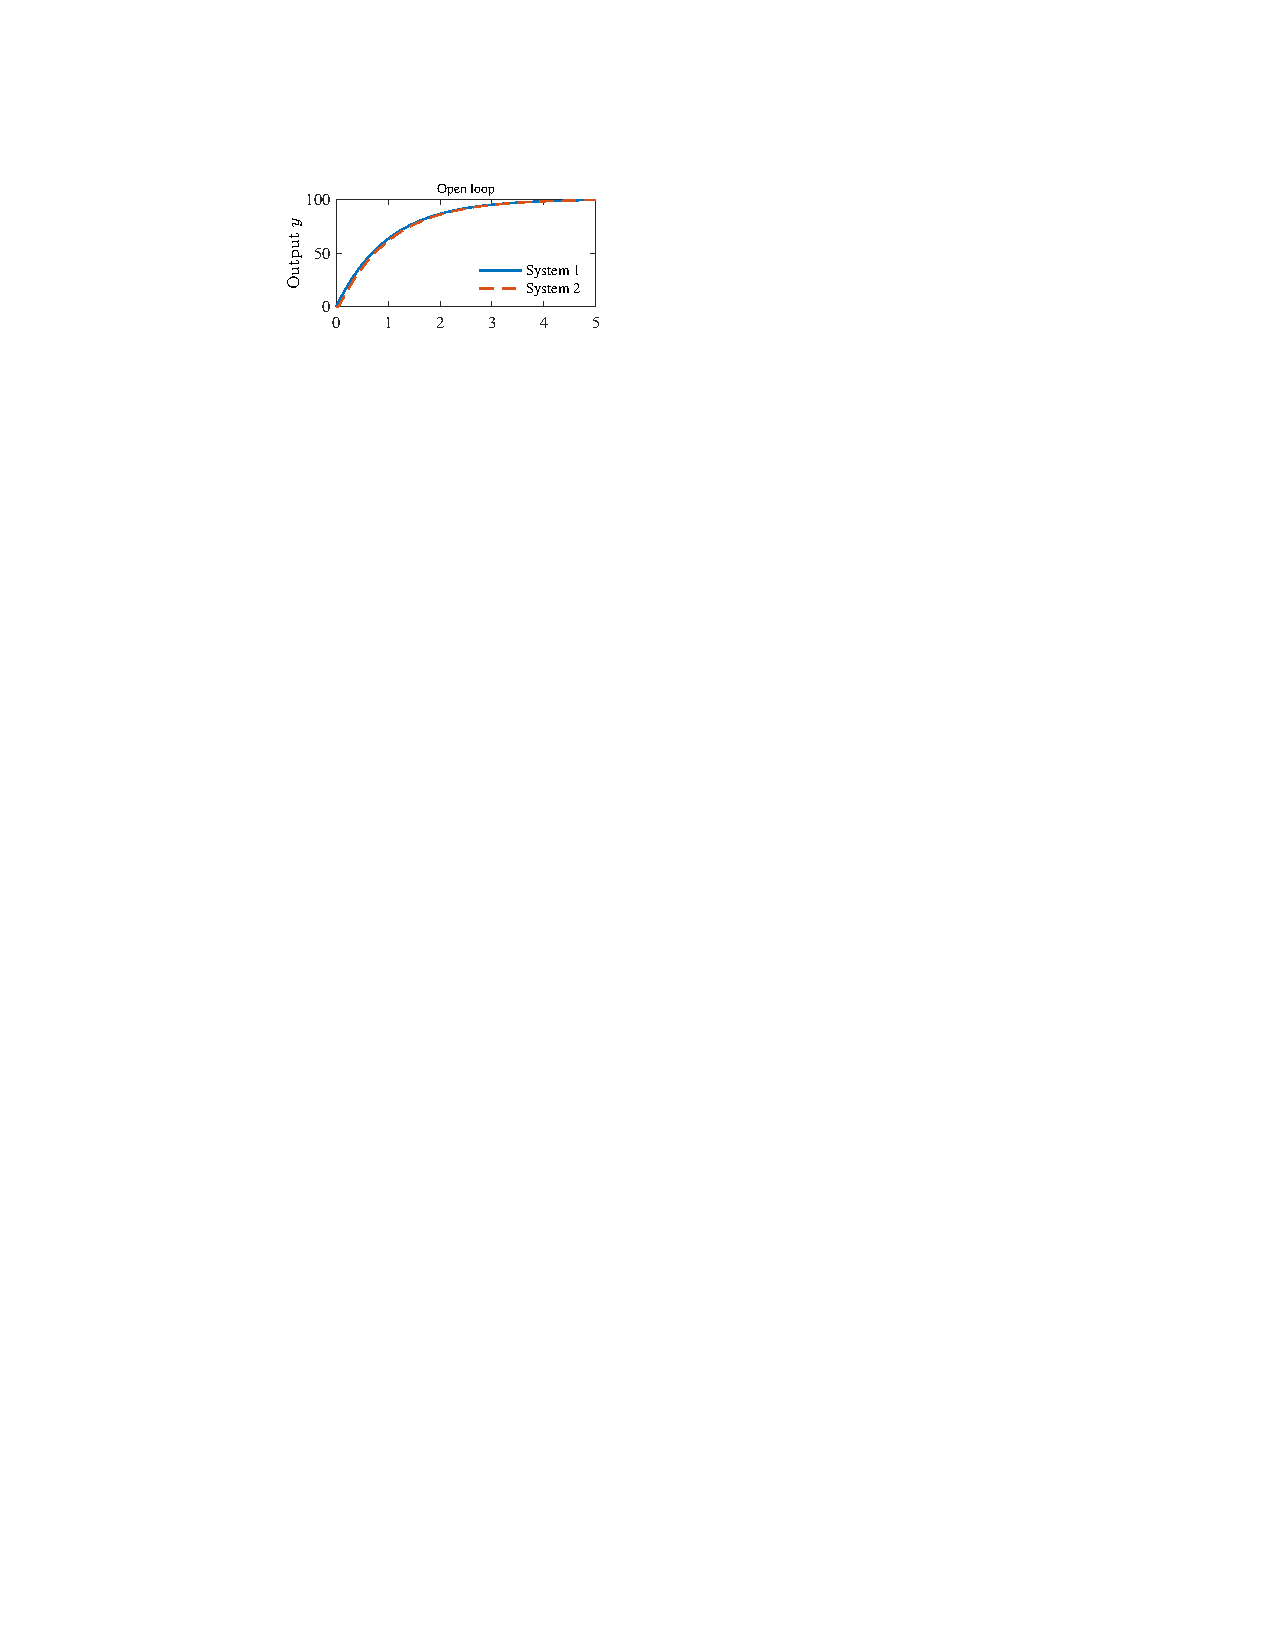
\includegraphics[width=4.5cm]{figure13.3a1} 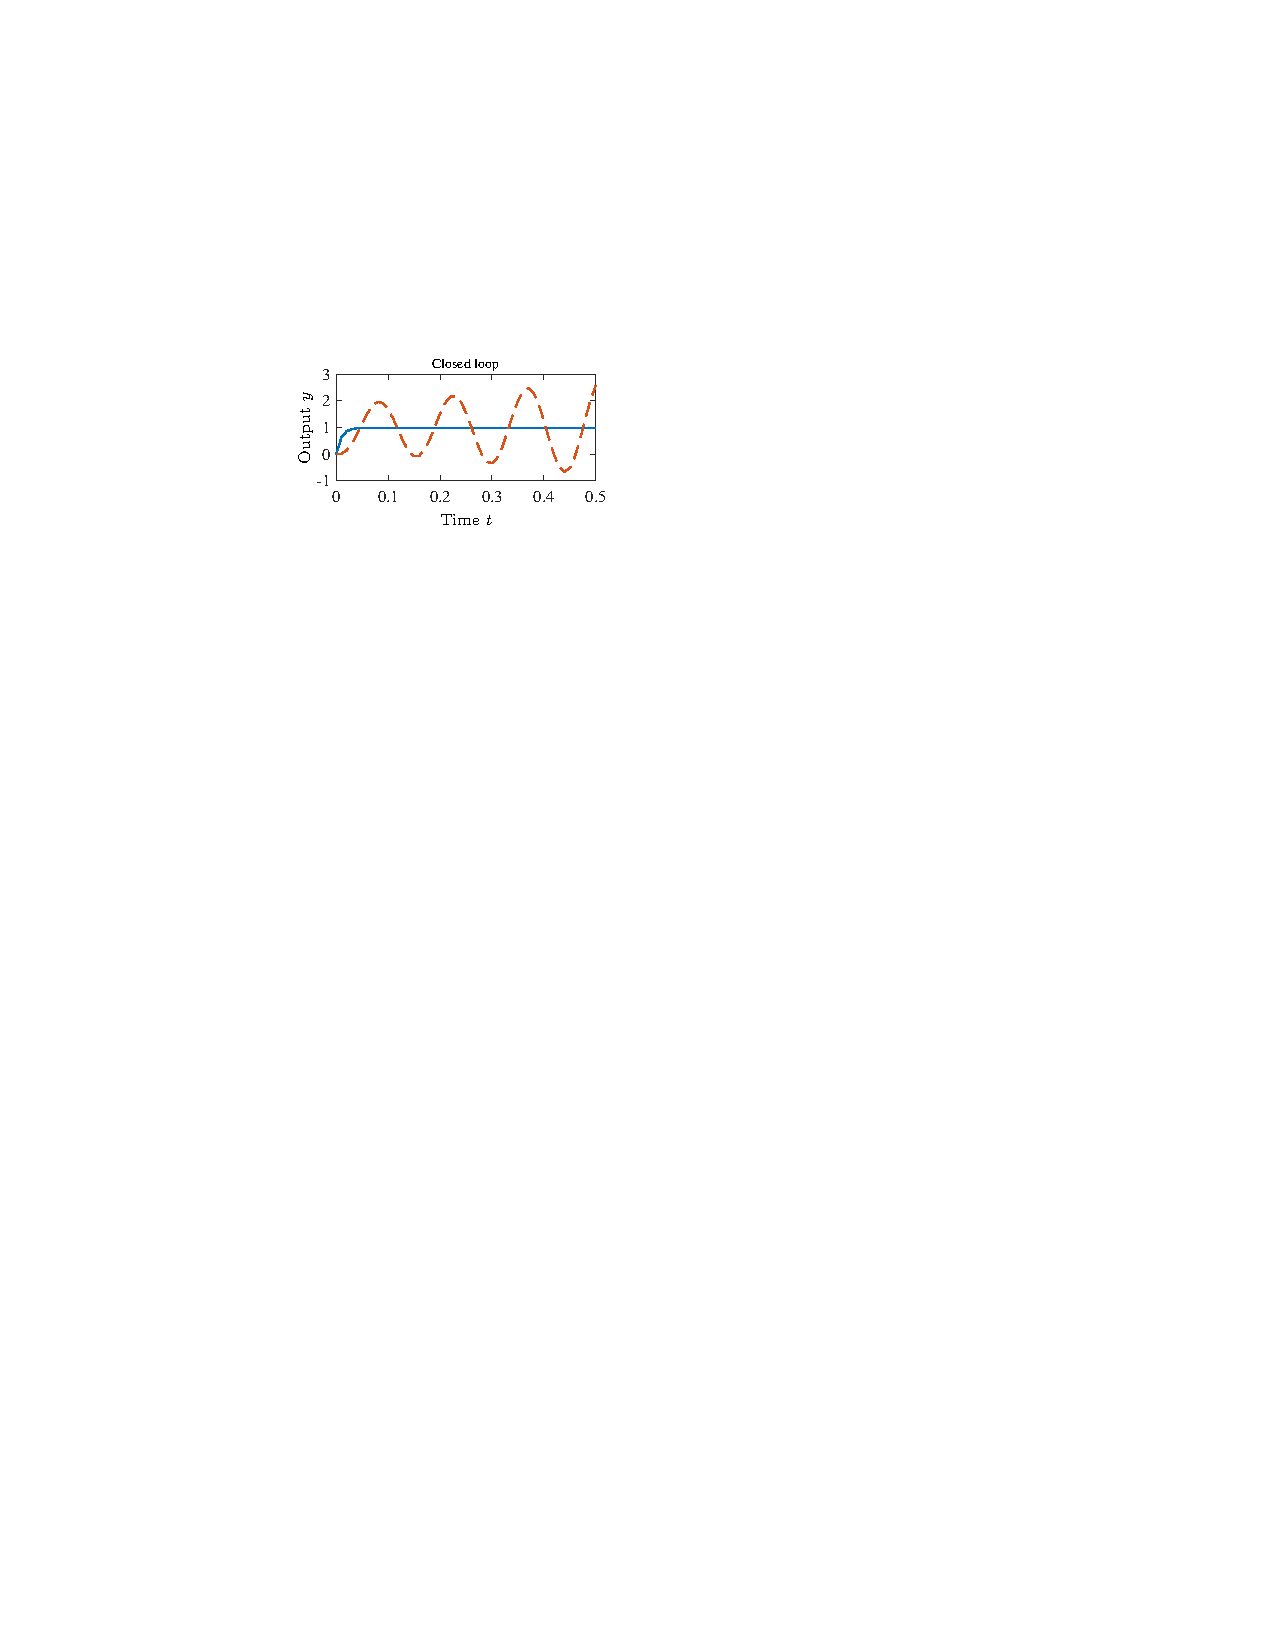
\includegraphics[width=4.5cm]{figure13.3a2} \\
	\vspace{-0.2cm}
	\textbf{Figure 13.3(a):} Determining when two systems are close $(T=0.025, k=100)$.
\end{figure}
\end{frame}


\begin{frame}{Examples}
	\begin{itemize}
		\item Consider the transfer functions 
		\[P_1(s)=\frac{k}{s+1},\quad P_2(s)=\frac{k}{s-1} \] 
		\item These systems are quite different in open loop
		\item Closing the loop as in the previous example shows that the two systems have very similar closed loop step responses for large $k$
		
	\end{itemize}
	\begin{figure}
		\centering
		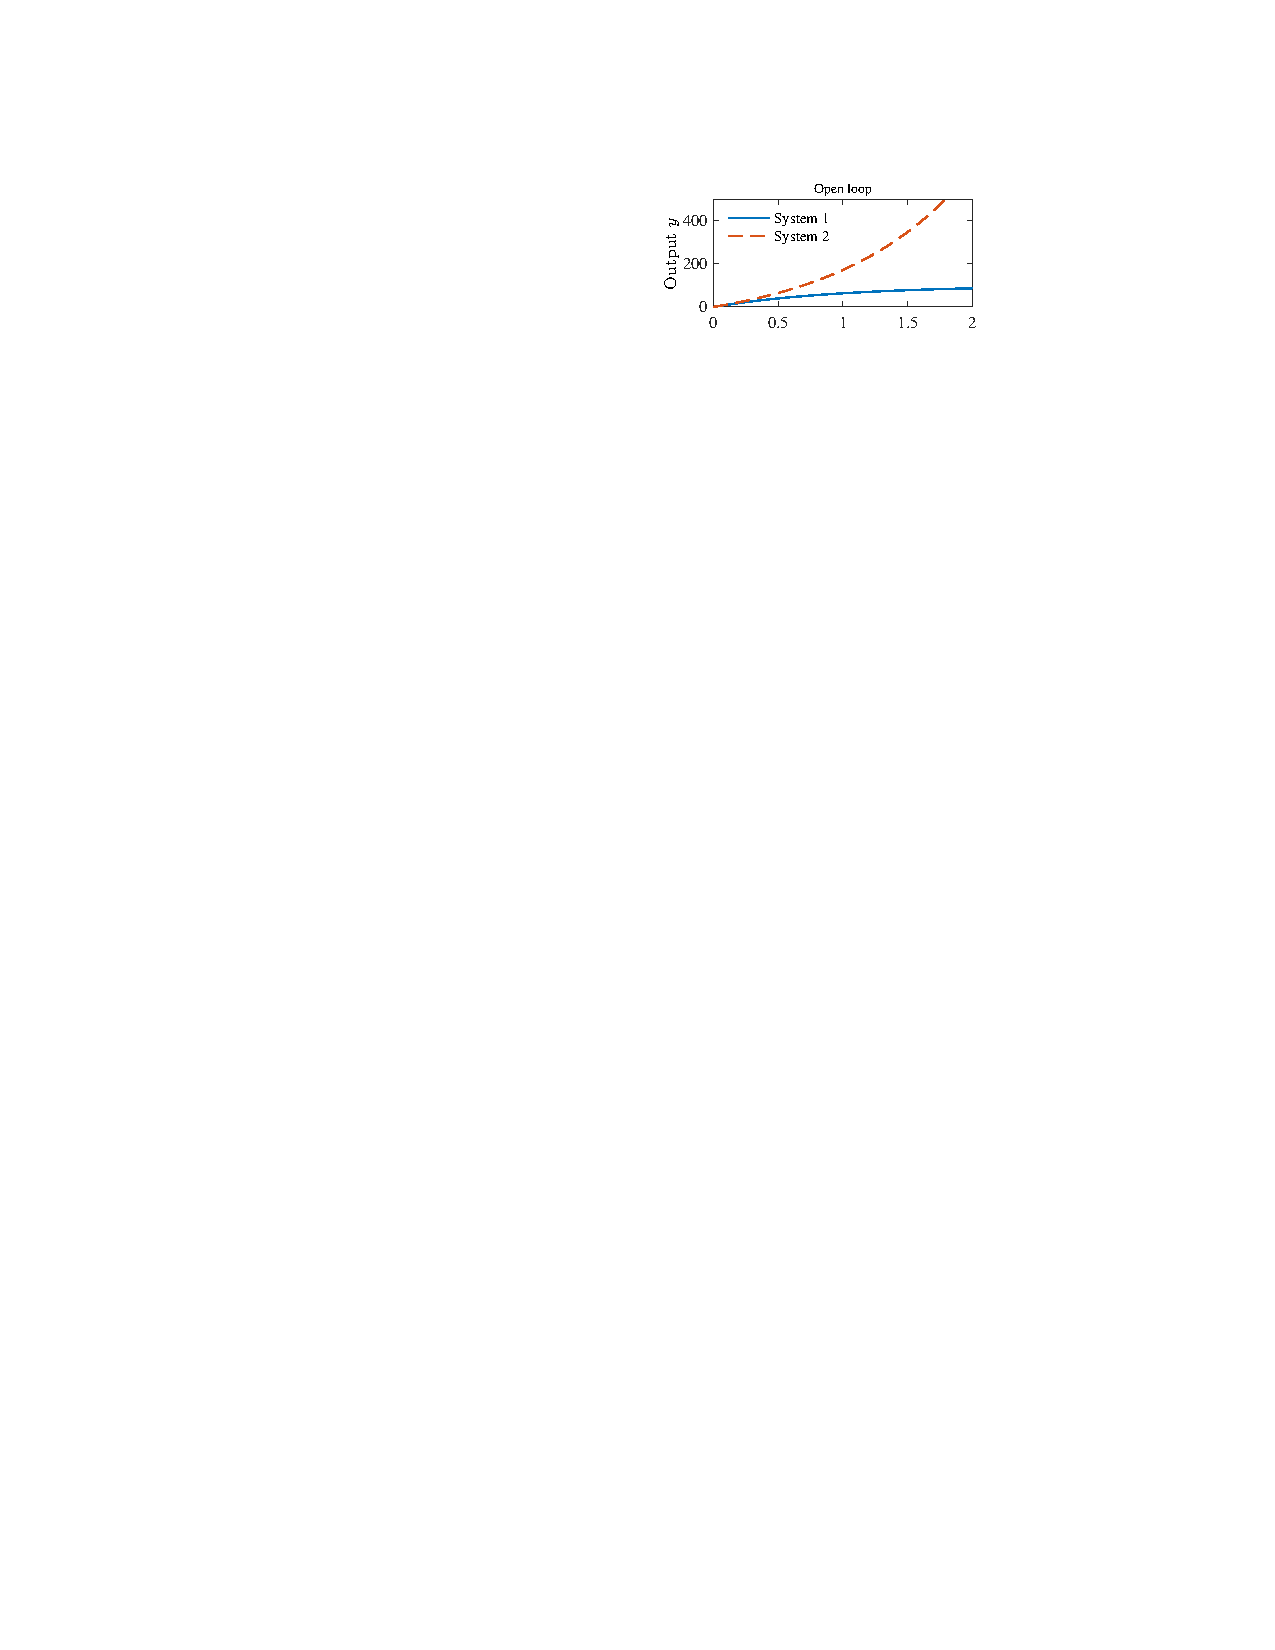
\includegraphics[width=4.5cm]{figure13.3b1} 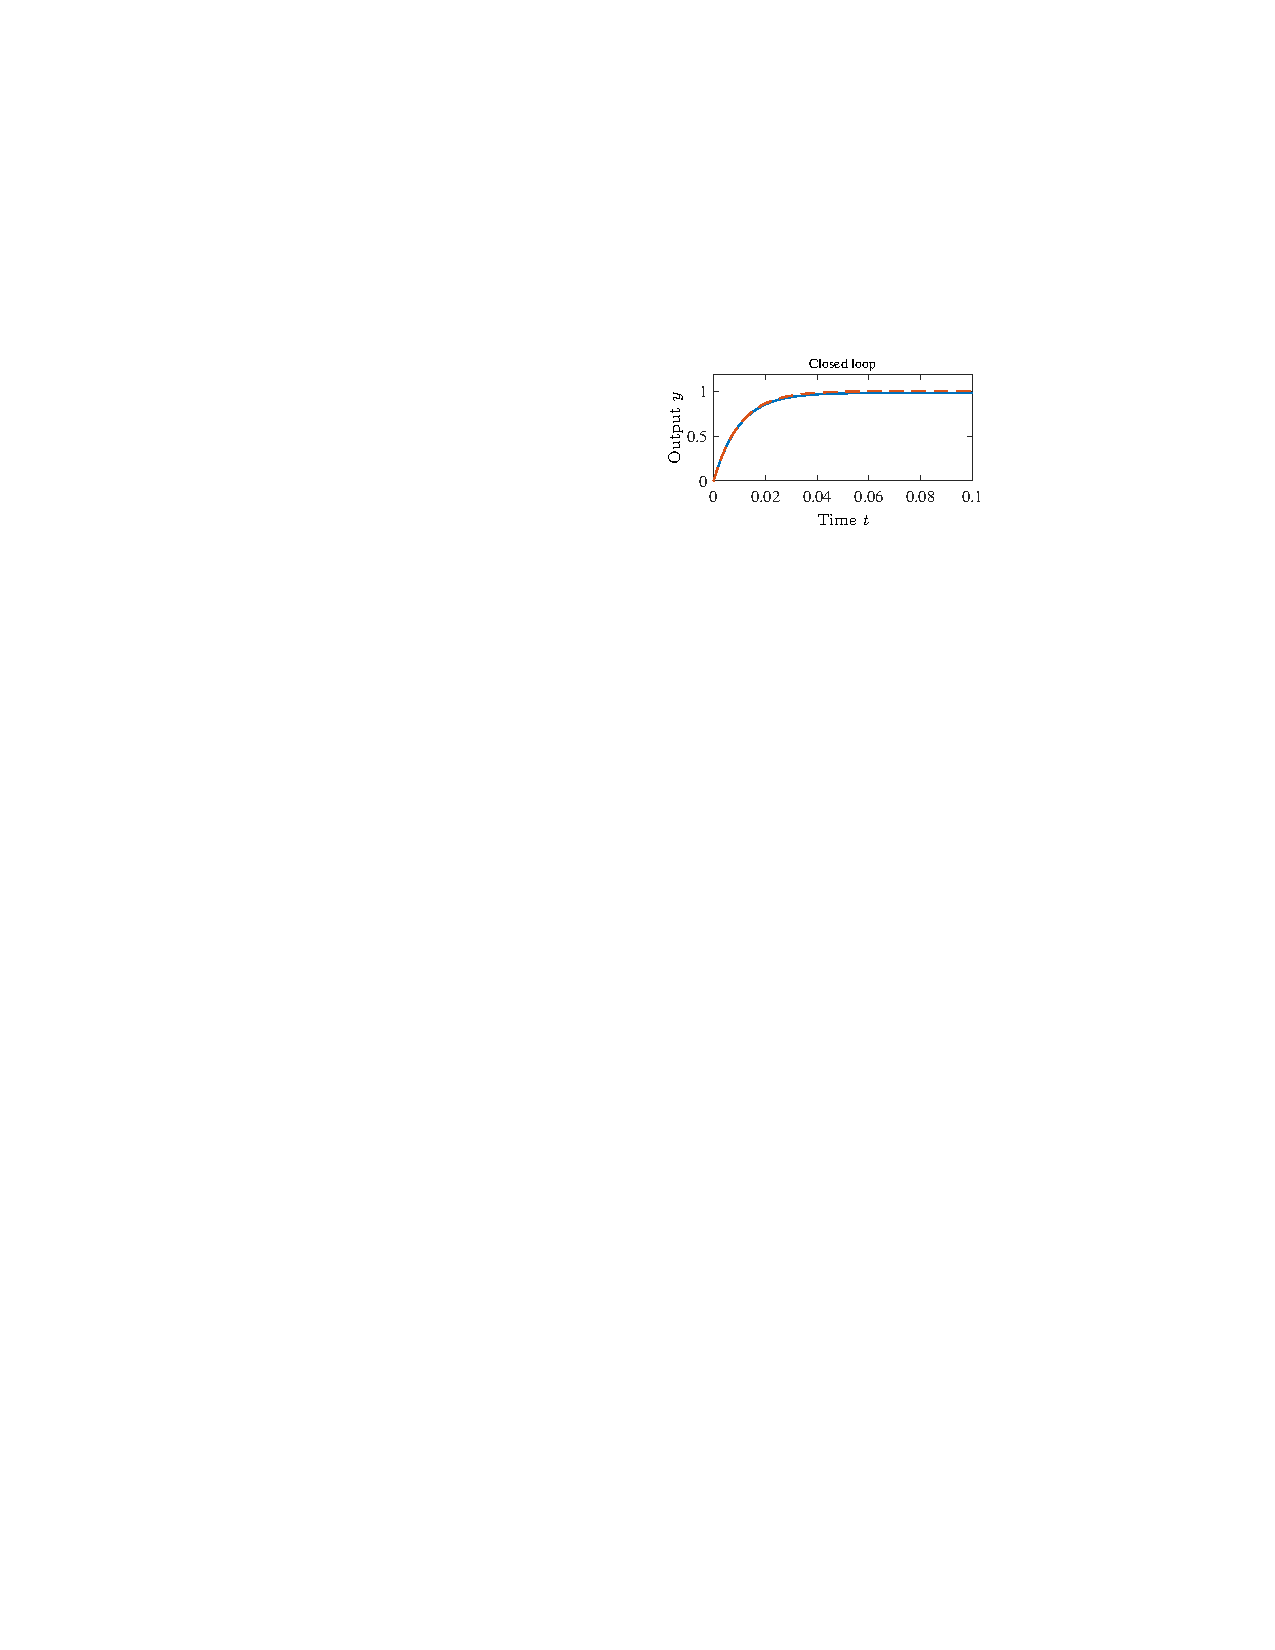
\includegraphics[width=4.5cm]{figure13.3b2} \\
		\vspace{-0.2cm}
		\textbf{Figure 13.3(b):} Determining when two systems are close $(k=100)$.
	\end{figure}
\end{frame}





\SUMMARYFRAME
\FINALE

\end{document}
